\section{GRE via Simulator Sets}\label{sec:simulation}

In this section we will discuss how to solve the $\+L$-GRE problem
using simulation. Given a model $\+M = \tup{\Delta,
\interp{\cdot}}$, Theorem~\ref{thm:simulation} tells us that if two
distinct elements $u$ and $v$ in $\Delta$ are such that $u
\simul{\+L} v$ then every $\+L$-formula that is true at $u$ is also
true at $v$. Hence there is no formula in $\+L$ that can uniquely
refer to $u$. From this perspective, knowing whether the model
contains an element that is $\gL$-similar but distinct from $u$ is
equivalent to decide whether there exists an $\+L$-RE for $u$.


Assume a fixed language $\+L$ and a model $\+M$.  Suppose we want to
refer to an element $u$ in the domain of $\+M$. We would like to
compute the \emph{simulator set} of $u$ defined as
$\simset_{\+L}^{\+M}(u) = \cset{v \in \Delta \mid u \simul{\+L} v}$.
When the model $\+M$ is clear from the context, we just write
$\simset_{\+L}$.
 If $\simset_{\+L}^{\+M}(u)$ is not the singleton $\cset{u}$,
the $\+L$-GRE problem with target $\{u\}$ in $\+M$ will fail.

\iffullversion
It is easy to see that the union of two $\+L$-simulations is
also an $\+L$-simulation. We can then define the \emph{maximal
auto $\+L$-simulation} (notation, $\simmax_{\+L}$) over a model $\+M$ as the union of all
auto $\+L$-simulations over $\+M$. Because
$\simset_{\+L}(u) = \cset{v \mid u \simmax_{\+L} v}$, an algorithm
for computing $\simmax_{\+L}$ also computes $\simset_{\+L}(u)$.
\else
\fi

\iffullversion
If $P$ is reflexive and transitive then so is $\simmax_P$. In
particular, $\simmax$ is reflexive and transitive.
\fixme{Are reflexivity and transitivity important? Check.}
\else
\fi



An algorithm is given in~\cite{HHK95} to compute $\simset_{\ELAN}(v)$ for each
element $v$ of a given finite model
$\+M=\tup{\Delta,\interp{\cdot}}$
%\footnote{%
%  Actually the algorithm proposed in \cite{HHK95} is over labeled graphs, but
%  it can be adapted to compute $\simset_{\ELAN}$ by
%  appropriately labeling the model.%
%}
in time $O(\size{\Delta}\times\size{{\interp{\cdot}}})$.
Intuitively, this algorithm
defines $S(v)$ as a set of candidates for simulating $v$ and
successively refines it by removing those which fail to
simulate $v$.
%Since we never put new vertices into $\simset(v)$, all the deletions
%from $\simset(v)$ are permanent.
In the end, $S(v)=\simset_\ELAN(v)$. The algorithm can be adapted to
compute $\simset_\+L$ for many other languages $\+L$. In particular,
we can use it to compute $\simset_\EL$ in polynomial time which will
give us the basic algorithm for establishing an upper bound to the
complexity of the \EL-GRE problem --this will answer an open
question of~\cite{AKS08}. The pseudo-code is shown in
Algorithm~\ref{alg:schematic-gen-sim}, which uses the following
notation: $\+P$ is a fixed set of unary relation symbols,  for $v\in
\Delta$, let $\unary(v)=\{p\in\+P\mid v\in\interp{p}\}$ and let also
$\su{r}{v}=\{u\in\Delta\mid(v,u)\in\interp{r}\}$ for $r$ a binary
relation symbol.

\begin{algorithm} \small
\caption{\small Computing \EL-similarity}\label{alg:schematic-gen-sim}
\SetKwInOut{Input}{input}\SetKwInOut{Output}{output}
\Input{a finite model $\+M=\tup{\Delta,\interp{\cdot}}$}
\Output{$\forall v\in \Delta$, the simulator set
$\simset_\EL^{\+M}(v)=S(v)$} \BlankLine

\ForEach{$v\in \Delta$}{$S(v):=\{u\in \Delta \mid \unary(v)
\subseteq \unary(u) \}$}

\While{\guard}{$S(u):=S(u)\setminus\{w\}$}
\end{algorithm}


%First some notation. For any $v\in \Delta$ and any binary relation
%$r$, let
%\begin{eqnarray*}
%\unary(v)&=&\{p\mid \mbox{$p$ is a unary rel.\ and
%$v\in\interp{p}$}\}\\
%%\pr{r}{v}&=&\{u\in\Delta\mid(u,v)\in\interp{r}\}\\
%\su{r}{v}&=&\{u\in\Delta\mid(v,u)\in\interp{r}\}
%\end{eqnarray*}
%%The last two extend to sets $V\subseteq\Delta$ as usual:
%%$\pr{r}{V}=\bigcup_{v\in V}\pr{r}{v}$ and $\su{r}{V}=\bigcup_{v\in
%%V}\su{r}{v}$.

%

The algorithm is fairly straightforward. We initialize $S(v)$ with
the set of all elements $u\in\Delta$ such that $\unary(v)\subseteq
\unary(u)$, i.e., the set of all elements satisfying at least the
same unary relations as $v$ (this guarantees that property $\atomL$ holds).
At each step, if there are three elements $u$, $v$ and $w$ such that
for some relation $r$, $(u,v) \in \interp{r}$, $w\in S(u)$
(i.e., $w$ is a candidate to simulate $u$) but $\su{r}{w}\cap S(v) = \emptyset$
(there is no element $w'$ such that $(w, w') \in \interp{r}$
and $w'\in S(v)$) then clearly condition $\zig$ is not satisfied
under the supposition that $\simset_\EL=S$. $S$ is `too big' because
$w$ cannot simulate $u$. Hence $w$ is removed from $S(u)$.

Algorithm~\ref{alg:schematic-gen-sim} will only tell us
whether an \EL-RE for an element $u$ exists (that is,
whether $\simset_{\EL}(u) = \cset{u}$ or not).  It does not compute
an \EL-formula $\varphi$ that uniquely refers to $v$. But
we can adapt it to obtain such a formula.
Algorithm~\ref{alg:schematic-gen-sim}'s main strategy to compute simulations
is to successively
refine an over-approximation of the simulator sets.
The ``reason'' behind each refinement  can be encoded using an \EL-formula.
Using this insight, one can transform an algorithm that computes
$\+L$-simulator sets with a similar strategy,  into one that additionally computes an $\+L$-RE
for each set.


Algorithm~\ref{alg:schematic-GRE} shows a transformed version of
Algorithm~\ref{alg:schematic-gen-sim} following this principle. The
idea is that each node $v\in\Delta$ is now tagged with a formula
$F(v)$ of \EL. The formulas $F(v)$ are updated along the execution of
the loop, whose invariant  ensures that $v \in
\interp{F(v)}$ and $\interp{F(u)} \subseteq S(u)$ hold for all
$u,v\in\Delta$.

\begin{algorithm}\small
%\LinesNumbered
\io

\ForEach{$v\in \Delta$}{ $S(v):=\{u\in \Delta \mid \unary(v)
\subseteq \unary(u) \}$\;\label{alg:line:init1}

$F(v):=\bigwedge \unary(v)$\;\label{alg:line:init2} }

\While{\guard}
{
 %$\{\ I: \mbox{\bf assert }(\forall u,v)\ \interp{F(u)} \subseteq S(u)\wedge v \in \interp{F(v)} \ \}$
 \KwSty{invariant} $\forall u,v: \interp{F(u)} \subseteq S(u)\wedge v \in \interp{F(v)}$\\
$S(u):=S(u)\setminus\{w\}$\;\label{alg:line:loop-body-begin}

\If{$\diam F(v)$ is not a conjunct of $F(u)$}{ $F(u):=F(u)\wedge
\diam F(v)$\;\label{alg:line:loop-body-end-1} }} \caption{\small
Computing $\EL$-similarity and \posre}\label{alg:schematic-GRE}
\end{algorithm}

Initially $F(v)$ is the conjunction of all the unary relations that
satisfy $v$ (if there is none, then $F(v)=\top$).
Each time the algorithm finds elements $r,u,v,w$
such that $(u,v)\in\interp{r}$, $w\in S(u)$ and $\su{r}{w}\cap
S(v)=\emptyset$, it updates $F(u)$ to $F(u)\wedge\diam F(v)$.
Again this new formula $\phi$ is in $\pos$ and it can be
shown that $v\in\interp{\phi}$ and $w\notin\interp{\phi}$, hence
witnessing that $v\simil{\EL} w$ is false.

%As we will see in Theorem~\ref{thm:correctness-schematic-GRE}, this
%formula is true in $v$ but false in $w$, hence witnessing that $w$
%does not simulate $v$.


%It is clear that Algorithm \ref{alg:schematic-GRE} terminates.

\iffullversion One wants to know whether a given set $V\subseteq W$
has an \posre. How do we interpret the output of Algorithm
\ref{alg:schematic-GRE}? Here is the answer: $V\subseteq W$ has an
\EL-RE iff there is a node $v\in V$ such that $V=\{u\in W\colon
v\in\simset_\subseteq(u) \wedge u\in\simset_\subseteq(v)\}$. In
other words, $V$ has an \EL-RE iff $V$ is the set of nodes which are
\emph{bisimilar} to some node of $V$. Here we say that $u$ and $v$
are \emph{bisimilar} if $u\in\simset_\subseteq(v)$ and
$v\in\simset_\subseteq(u)$. In case $V=\{v_1,\dots,v_n\}$ has an
\posre, any $F(v_i)$ is a valid \posre, so one can pick any of them.

In particular, $v$ has an \EL-RE if and only if $\simset_\subseteq(v)=\{v\}$
and in case $v$ has a \EL-referring expression then $F(v)$ is a
valid one. If $v$ does not have an \posre then the algorithm may be
used to approximate an \posre. Indeed, since every formula true at
$v$ is also true at all nodes in $\simset_\subseteq(v)$ and $F(v)$
is true at every node of $\simset_\subseteq(v)$ then $F(v)$ is a
reasonable approximation of an \EL-RE for $v$.

\begin{ex}
Let $\gG$ be the following model
\begin{center}
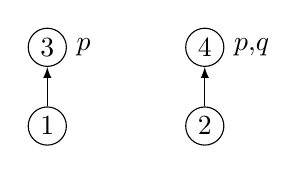
\begin{tikzpicture}[>=latex]
  \node (n1) at (0,0) [shape=circle,draw,inner sep=2pt, label=right:$$] {$1$} ;
  \node (n2) at (2,0) [shape=circle,draw,inner sep=2pt, label=right:$$] {$2$} ;
  \node (n4) at (0,1) [shape=circle,draw,inner sep=2pt, label=right:$p$] {$3$} ;
  \node (n5) at (2,1) [shape=circle,draw,inner sep=2pt, label=right:$p{,}q$] {$4$} ;
  \draw [->] (n1) -- (n4);
  \draw [->] (n2) -- (n5);
\end{tikzpicture}
\end{center}
%
where $\rg\ l=\cset{p,q}$ and the valuation is defined as
$l(3)=\cset{p}, l(4)=\cset{p,q}, l(1)=l(2)=\cset{}$. The initial values of $S$ and $F$ are
shown in Table~\ref{tab:example}.

\begin{table}[ht]
\centering
{\footnotesize
\begin{tabular}{|c|c|c|c|c|}
\hline
&\multicolumn{2}{|c|}{Initial}&\multicolumn{2}{|c|}{Final}\\
$v$ & $S(v)$ & $F(v)$ & $S(v)$&$F(v)$\\
\hline
$1$ & $\{1,2,3,4\}$ & $\top$ & $\{1,2\}$&$\top\wedge\diam p$\\
$2$ & $\{1,2,3,4\}$ & $\top$ & $\{2\}$&$\top\wedge\diam(p\wedge q)$\\
$3$ & $\{3,4\}$ & $p$ & $\{3,4\}$ &$p$\\
$4$ & $\{4\}$ & $p\wedge q$ & $\{4\}$&$p\wedge q$\\
\hline
\end{tabular}
\caption{Initial and final values of $F$ and $S$}\label{tab:example}
}
\end{table}

Suppose the following execution:
\begin{enumerate}
\item Choose $u=2,v=4,w=1$: detect that $1$ does not simulate $2$; set $S(2)=\{2,3,4\}$ and $F(2)=\top\wedge\diam(p\wedge q)$
\item Choose $u=2,v=4,w=3$: detect that $3$ does not simulate $2$; set $S(2)=\{2,4\}$ and $F(2)=\top\wedge\diam(p\wedge q)$
\item Choose $u=2,v=4,w=4$: detect that $4$ does not simulate $2$; set $S(2)=\{2\}$ and $F(2)=\top\wedge\diam(p\wedge q)$
\item Choose $u=1,v=3,w=3$: detect that $3$ does not simulate $1$; set $S(1)=\{1,2,4\}$ and $F(1)=\top\wedge\diam p$
\item Choose $u=1,v=3,w=4$: detect that $4$ does not simulate $1$; set $S(1)=\{1,2\}$ and $F(1)=\top\wedge\diam p$
\end{enumerate}
After the fifth iteration it terminates. The final output is shown
in Table~\ref{tab:example}. From this output one may conclude that,
since $\simset_\subseteq(4)=\{4\}$, node $4$ has an \posre, namely
$p\wedge q$. Node $2$ also has the \EL-RE $\top\wedge\diam(p\wedge
q)$. In contrast $3$ does not have an \EL-RE because every
$\pos$-formula true at $3$ is also true at $4$ (in this case, the
only such possible formula is $p$ itself, or logically equivalent
formulas such as $\top\wedge p\wedge p$). Nor $3$ has an \posre.
\end{ex}
\fi

\iffullversion
\begin{theorem}\label{thm:correctness-schematic-GRE}
Let $S$ and $F$ be the output of the Algorithm
\ref{alg:schematic-GRE} with input $\gG=\tup{N,\to,l}$. Then for each
node $v\in N$, $\interp{F(v)} = S(v) = \simset_\subseteq(v)$
\end{theorem}
\fi

\iffullversion
\begin{proof}
It is clear that for each node $v\in N$,
$\simset_\subseteq(v)=S(v)$. For the second part, we propose the
following invariant for the main loop:
\begin{itemize}
\item[$I_1$:] for each $v\in N$, $v \in \interp{F(v)}$
\item[$I_2$:] for each $u,v\in N$, $\interp{F(u)} \subseteq S(u)$
\end{itemize}
Let us analyze the state after the initialization, before line~\ref{alg:line:loop-begin} is executed for the fist time. On the one
hand, it is clear that for any node $v\in N$, $v \in \interp{F(v)}$, so
$I_1$ is verified. On the other, if $v\notin S(u)$ then
$l(u)\not\subseteq l(v)$ and so there is a propositional symbol
$p$ such that $p \in l(u)$ and $p \notin l(v)$. Since $v\notin\interp{p}$
then $v\notin\interp{\bigwedge l(u)}$ and therefore
$v\notin \interp{F(u)}$.

Suppose that $I_1$ and $I_2$ are true before executing
line~\ref{alg:line:loop-body-begin}. For all $v\in N$ let $S(v)=S_v$ and
$F(v)=\phi_v$ in this state. Let $u,v,w$ be the chosen nodes. We
show that the invariant is reestablished after executing line
\ref{alg:line:loop-body-end-1}. Since $F$ and $S$ only change for $u$,
it suffices to show
\begin{itemize}
\item[$I_1'$:] $u \in \interp{\phi_u\wedge\diam \phi_v}$
\item[$I_2'$:] $\forall v\in N, \interp{\phi_u\wedge\diam \phi_v} \subseteq S_u\setminus\{w\}$
\end{itemize}
For $I_1'$, it is clear from $I_1$ that $u \in \interp{\phi_u}$ and
$v \in \interp{\phi_v}$. Since $u\to v$ we conclude $u \in \interp{\diam
\phi_v}$.

For $I_2'$ we show that for any $v$, if $v\notin S_u\setminus\{w\}$
then $v\notin \interp{\phi_u\wedge\diam \phi_v}$. If $v\notin S_u$,
by $I_2$ we know $v\notin \interp{\phi_u}$ and therefore $v\notin
\interp{\phi_u\wedge\diam \phi_v}$. Suppose $v=w$ and, by
contradiction, assume $v \in \interp{\phi_u\wedge\diam \phi_v}$.
Then there is $w'\in N$ such that $v\to w'$ and $w' \in
\interp{\phi_v}$. By $I_2$ this implies $w'\in S_v$. Hence
$w'\in\su(w)\cap S_v$ and this contradicts the choice of $u,v,w$.

When the algorithm terminates, $S=\simset_\subseteq$ and therefore
the invariant $I_2$ implies that for each $u,v\in N$,
$F(u) \subseteq \simset_\subseteq(u)$. On the other hand, $I_1$
implies that $u \in \interp{F(u)}$ and by Proposition \ref{prop:equiv} we
have that if $v\in \simset_\subseteq(u)$ then $v \in \interp{F(u)}$.
Therefore for each $u,v\in N$, $\interp{F(u)} = \simset_\subseteq(u)$. So defining $\form:=F$ we obtain the desired result.
\end{proof}
\else
\fi

\iffullversion
\begin{theorem}
Algorithm~\ref{alg:schematic-GRE} with input $\gG = \tup{N,\to,l}$
terminates in time
$O(\size{{\to}}^2\cdot\size{N}^3+\size{N}\cdot\size{\rg\ l})$.
\end{theorem}
\fi

\iffullversion
\begin{proof}
For a naive implementation, the main loop executes at most
$\size{N}^2$ may times and to find $u,v,w$ in
line~\ref{alg:line:loop-begin} we need $O(\size{N}\cdot\size{{\to}}^2)$
many steps. The running time of the loop body is absorbed by this
last quantity. Hence, in total, the execution time of the main loop
is $O(\size{{\to}}^2\cdot\size{N}^3)$. For each $v\in N$, we need
$O(\size{\rg\ l})$ many steps for lines~\ref{alg:line:init1} and~\ref{alg:line:init2}. So in total, the initialization takes
$O(\size{N}\cdot\size{\rg\ l})$ many steps.
\end{proof}
\else
\fi

\iffullversion
\begin{algorithm} \small
\io

\ForEach{$v\in \Delta$}{ $\prevS(v):=\Delta$

\If{for all binary $r$, $\su{r}{v}=\emptyset$}{$S(v):=\{u\in \Delta
\mid \unary(v)\ \subseteq \unary(u) \}$

$F(v):=\bigwedge\unary(v)$ } \Else{ let $r$ be a binary relation
such that $\su{r}{v}\not=\emptyset$

 $S(v):=\{u\in \Delta \colon
\unary(v) \subseteq \unary(u)\wedge\su{r}{u}\not=\emptyset \}$

$F(v):=\diam\top\wedge\bigwedge P(v)$ }}

\While{$\exists\ v\in \Delta:S(v)\not=\prevS(v)$}{

$\{\ I_1:\mbox{\bf assert\ }(\forall v)\ S(v)\subseteq\prevS(v)\ \}$

$\{\ I_2:\mbox{\bf assert\ }(\forall r,u,v,w)\
[(u,v)\in\interp{r}\wedge w\in
S(u)]\Rightarrow[\su{r}{w}\cap\prevS(v)\not=\emptyset]\ \}$

\ForEach{\mbox{\rm binary relation $r$ and $u\in \pr{r}{v}$}}{

$remove := \pr{r}{\prevS(v)}\setminus\pr{r}{S(v)}$

$S(u):=S(u)\setminus remove$

\If{$\diam F(v)$ is not a conjunct of $F(u)$}{ $F(u):=F(u)\wedge
\diam F(v)$\label{alg:line:loop-body-end-2} } }

$\prevS(v)=S(v)$

} \caption{\small refined $\EL$-similarity and
\posre}\label{alg:refined-GRE}
\end{algorithm}
\fi

Algorithm \ref{alg:schematic-GRE} can be easily modified to
calculate the \ELAN-RE of each simulator set $\simset_{\ELAN}$ by
adjusting the initialization: replace $\subseteq$ by $=$ in the
initialization of $S(v)$ and initialize $F(v)$ as
$\bigwedge\left(\unary(v)\cup\overline \unary(v)\right)$,
where $\overline \unary(v)=\{\lnot p\mid v\notin\interp{p}\}$.


With a naive implementation Algorithm~\ref{alg:schematic-GRE}
executes in time $O(\size{\Delta}^3\times$
$\size{\interp{\cdot}}^2)$
%\fixme{Santi: chequear la complejidad}
providing a polynomial solution to the \EL and \ELAN-GRE problems.
Algorithm~\ref{alg:schematic-gen-sim} can be transformed to run with a lower complexity
as in shown in~\cite{HHK95}; moreover this version of the algorithm can be adapted to
compute \EL- and \ELAN-RE for an arbitrary subset of the domain of $\tup{\Delta,\interp{\cdot}}$
 in $O(\size{\Delta}\times\size{\interp{\cdot}})$ steps. We shall skip the details.


%Given $\gG = \tup{N,\to,l}$,
%the
%
%$F$, the set of \posre, and $S$, the simulator sets s.t.\ $(\forall
%v\in \Delta)\ \interp{F(v)}=S(v)=\simset_\EL(v)$

%
\begin{theorem}\label{thm:complexity-EL-GRE}
The \EL and \ELAN-GRE problems over $\gM=\tup{\Delta,\interp{\cdot}}$ have complexity
$O(\size{\Delta}\times\size{\interp{\cdot}})$.
\end{theorem}

Theorem~\ref{thm:complexity-EL-GRE} answers a question left open
in~\cite{AKS08}: the \EL-GRE problem can be solved in polynomial
time. Note, however, that this  result assumes a convenient representation of
formulas like, for example, directed acyclic graphs, to ensure that
each step of the formula construction can be done in $O(1)$. In
\sect{size} we will take a closer look at the issue and its relation to
the size of the smallest $\+L$-RE.


%Theorem~\ref{thm:complexity-EL-GRE} shows that there are efficient
%GRE algorihtms for \EL and \ELAN; languages which are --as discussed
%in \sect{choosinglanguage}-- generally simple to realize. The
%methods presented here, together with previous results
%of~\cite{AKS08} indicate that algorithms for computing
%$\+L$-simulator sets can, in many cases, be adapted to solve the
%$\+L$-GRE problem at no extra complexity cost.


Algorithm~\ref{alg:schematic-GRE} was obtained by adding formula annotations
to a standard `\EL-simulation-minimization' algorithm. Given an
$\+L$-simulation-minimization, we can typically adapt it in an analogous
way to obtain an $\+L$-GRE algorithm.
The obtained algorithm computes $\+L$-REs for \emph{every} element of the
domain simultaneously.
This will make it particularly suitable for applications with
static domains requiring references to many objects.
% but given its low complexity
%and the fact that termination is ensured (no risk of infinite regression, see~\cite{dale91:_gener_refer_expres_invol_relat}),
%it seems suitable for most applications.
 Moreover, the algorithm can be adapted
to dynamic domains by using techniques used to recompute simulations (see~\cite{saha:incre07}),
so that only those RE that were affected by a change in the domain need to be
recomputed.

We have not addressed so far other relevant issues of the
GRE problem besides computational complexity. In particular,
Algorithm~\ref{alg:schematic-GRE} pays no attention to the use of
preferences among relations when generating an RE (i.e., preferring
the selection of certain attributes over others, when possible).
While there is room for improvement (e.g., making a weighted choice
instead of the non-deterministic choice when choosing elements
in the main loop of the algorithm), support for preferences is not
one of the strong points of this family of algorithms.
We consider algorithms with strong support for preferences in the following section.
